In diesem abschließenden Kapitel möchten wir nun die in
\Cref{chap:implementation} beschriebene Realisierung von
\Cref{alg:primalDualIteration} mit Abbruchkriterium
\eqref{eq:terminationCriterion} im Solve-Schritt der AFEM-Schleife aus
\Cref{fig:afemLoop} an einigen Benchmark-Problemen untersuchen.
Dabei konstruieren wir Probleme, bei denen die exakte Lösung bekannt ist,
nach \Cref{sec:constructionInputSignal}. 
Als besonderes Augenemerk betrachten wir dabei zwei Eingangssignale.
Andere Funktionen werden wir bei Bedarf betrachten, um bestimmte Eigenschaften
zu untersuchen im Vergleich zu diesen beiden Benchmark-Problemen.
Für ein Experiment mit exakter Lösung betrachten wir zunächst auf $[0,\infty)$
für einen Parameter $\beta\geq 1/2$, wobei wir stets $\beta =1$ wählen, 
die Funktionen
\begin{align*}
  u_1(r)&\coloneqq
  \begin{cases}
    1, 
    & \text{falls } r\in \left[0,\frac{1}{6}\right],\\
    1+(6r-1)^\beta, 
    & \text{falls } r\in \left(\frac{1}{6}, \frac{1}{3}\right],\\
    2, 
    & \text{falls } r\in \left(\frac{1}{3}, \frac{1}{2}\right],\\
    2\left(\frac{5}{2}-3r\right)^\beta, 
    & \text{falls } r\in \left(\frac{1}{2}, \frac{5}{6}\right],\\
    0, 
    & \text{falls } r\in \left(\frac{5}{6}, \infty\right),\\
  \end{cases}\\
  \sgn\big(\partial_r u_1(r)\big) 
  &\coloneqq
  \begin{cases}
    12r-36r^2, 
    & \text{falls } r\in \left[0,\frac{1}{6}\right],\\
    1, 
    & \text{falls } r\in \left(\frac{1}{6}, \frac{1}{3}\right],\\
    \cos(\pi(6r-2)), 
    & \text{falls } r\in \left(\frac{1}{3}, \frac{1}{2}\right],\\
    -1, 
    & \text{falls } r\in \left(\frac{1}{2}, \frac{5}{6}\right],\\
    -\frac{1+\cos(\pi(6r-5))}{2}, 
    & \text{falls } r\in \left(\frac{5}{6}, \infty\right).
  \end{cases}
\end{align*}
Nach \Cref{eq:constructionInputSignal} ist $u$ mit dieser Wahl von
$\sgn\big(\partial_r u_1\big)$ die Lösung von \Cref{prob:continuousProblem} mit
Eingangssignal
\begin{align*}
  f_1(r)
  &=
  \begin{cases}
    \alpha-12(2-9r), 
    & \text{falls } r\in \left[0,\frac{1}{6}\right],\\
    \alpha\left(1+(6r-1)^\beta\right)-\frac{1}{r}, 
    & \text{falls } r\in \left(\frac{1}{6}, \frac{1}{3}\right],\\
    2\alpha+6\pi\sin(\pi(6r-2))-\frac{1}{r}\cos(\pi(6r-2)), 
    & \text{falls } r\in \left(\frac{1}{3}, \frac{1}{2}\right],\\
    2\alpha\left(\frac{5}{2}-3r\right)^\beta+\frac{1}{r},
    & \text{falls } r\in \left(\frac{1}{2}, \frac{5}{6}\right],\\
    -3\pi\sin(\pi(6r-5))+\frac{1+\cos(\pi(6r-5))}{2r}, 
    & \text{falls } r\in \left(\frac{5}{6}, \infty\right).
  \end{cases}
\end{align*}

\begin{figure}[!ht]
  \centering
  \begin{subfigure}[b]{.48\linewidth}
    \caption{$f_1$}
    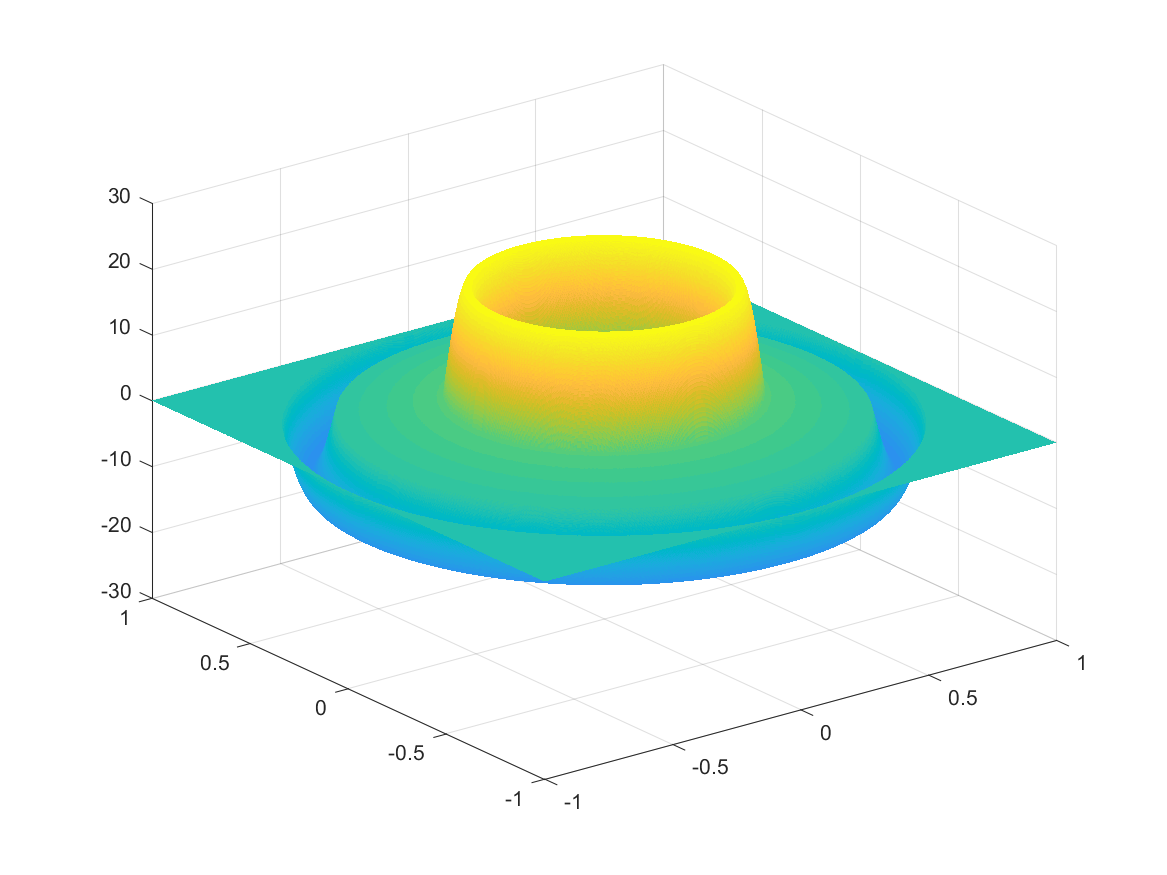
\includegraphics[trim = 40 30 30 30, clip, width=\linewidth]
      {pictures/chapExperiments/secGeneralInfo/f01Plots/inSi.png}
    \label{fig:f01InSi}
  \end{subfigure}
  \quad
  \begin{subfigure}[b]{.48\linewidth}
    \caption{$u_1$}
    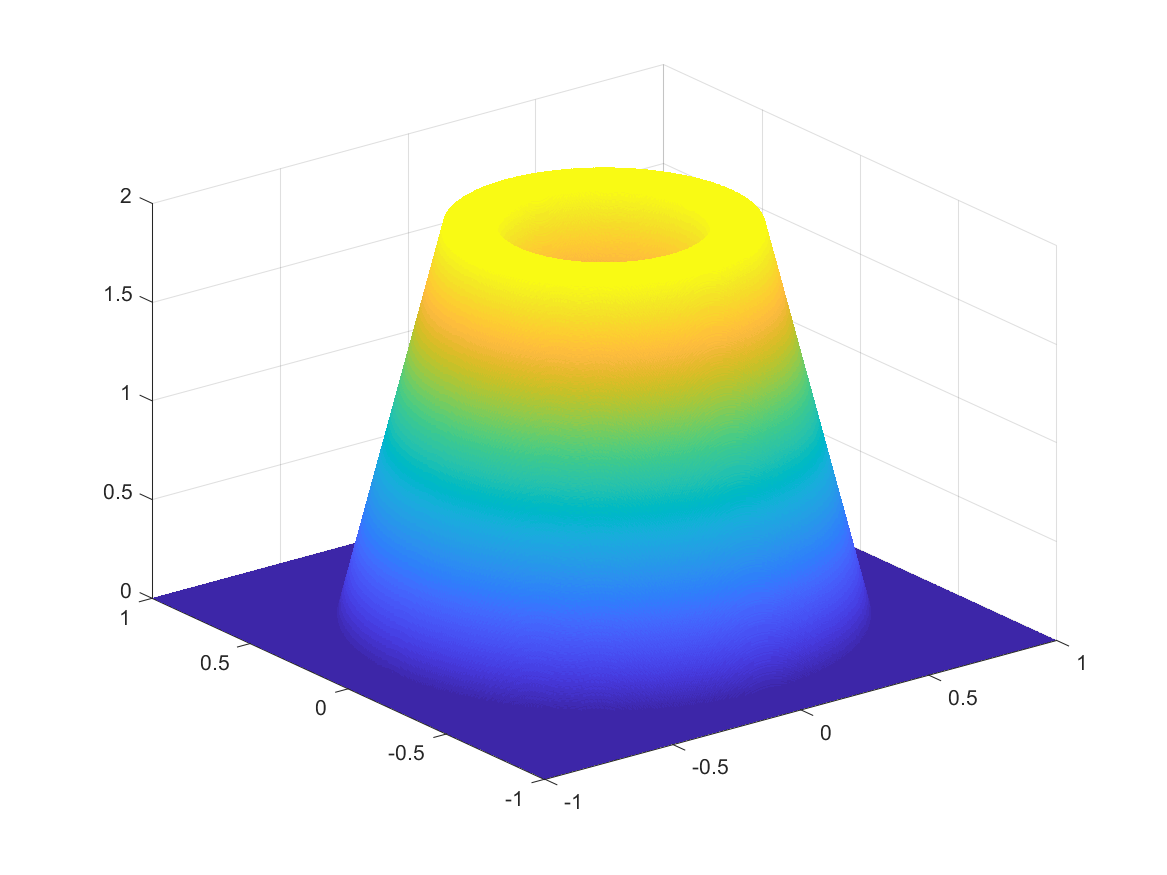
\includegraphics[trim = 40 30 30 30, clip, width=\linewidth]
      {pictures/chapExperiments/secGeneralInfo/f01Plots/exactSolution.png}
    \label{fig:f01ExactSol}
  \end{subfigure}

  \begin{subfigure}[b]{.48\linewidth}
    \caption{$f_1$ entlang der x- und y-Achse}
    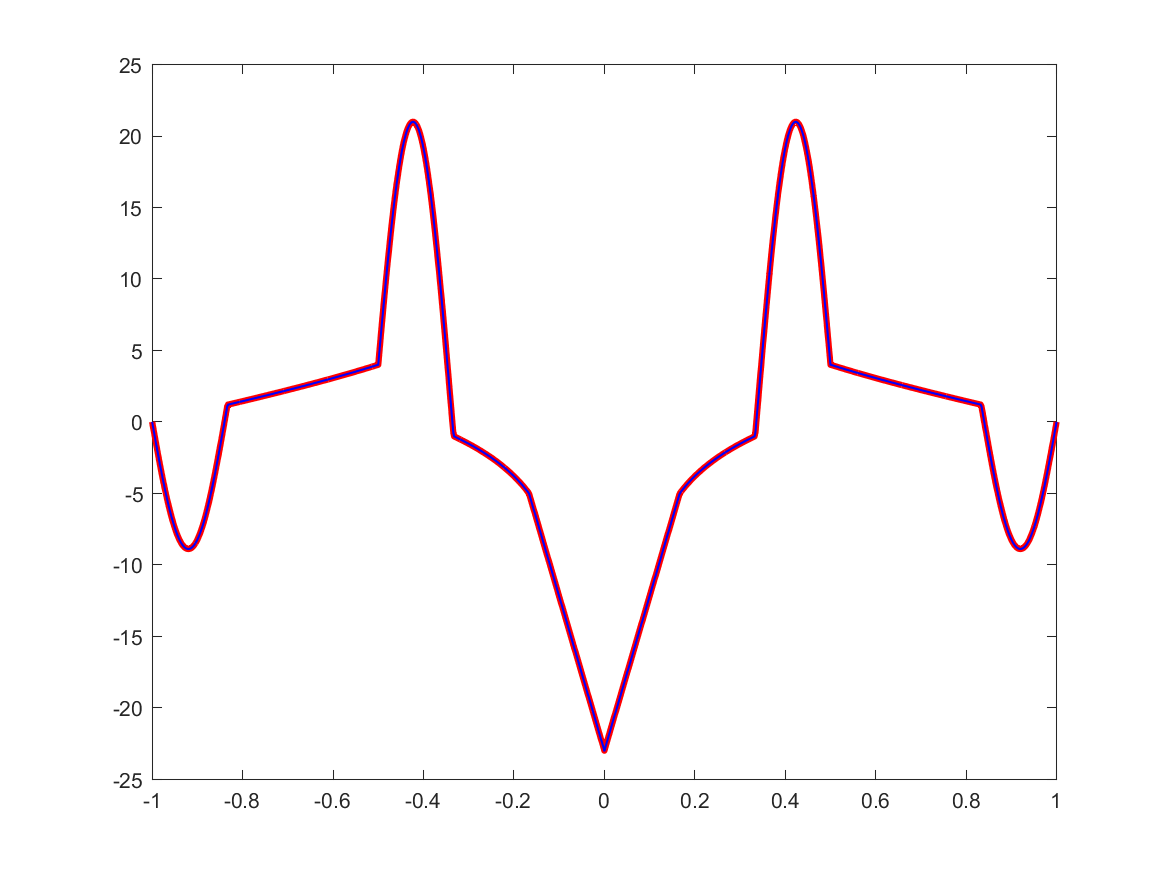
\includegraphics[trim = 50 30 50 20, clip, width=\linewidth]
      {pictures/chapExperiments/secGeneralInfo/f01Plots/inSiAxis.png}
    \label{fig:f01InSiAxis}
  \end{subfigure}
  \quad
  \begin{subfigure}[b]{.48\linewidth}
    \caption{$u_1$ entlang der x- und y-Achse}
    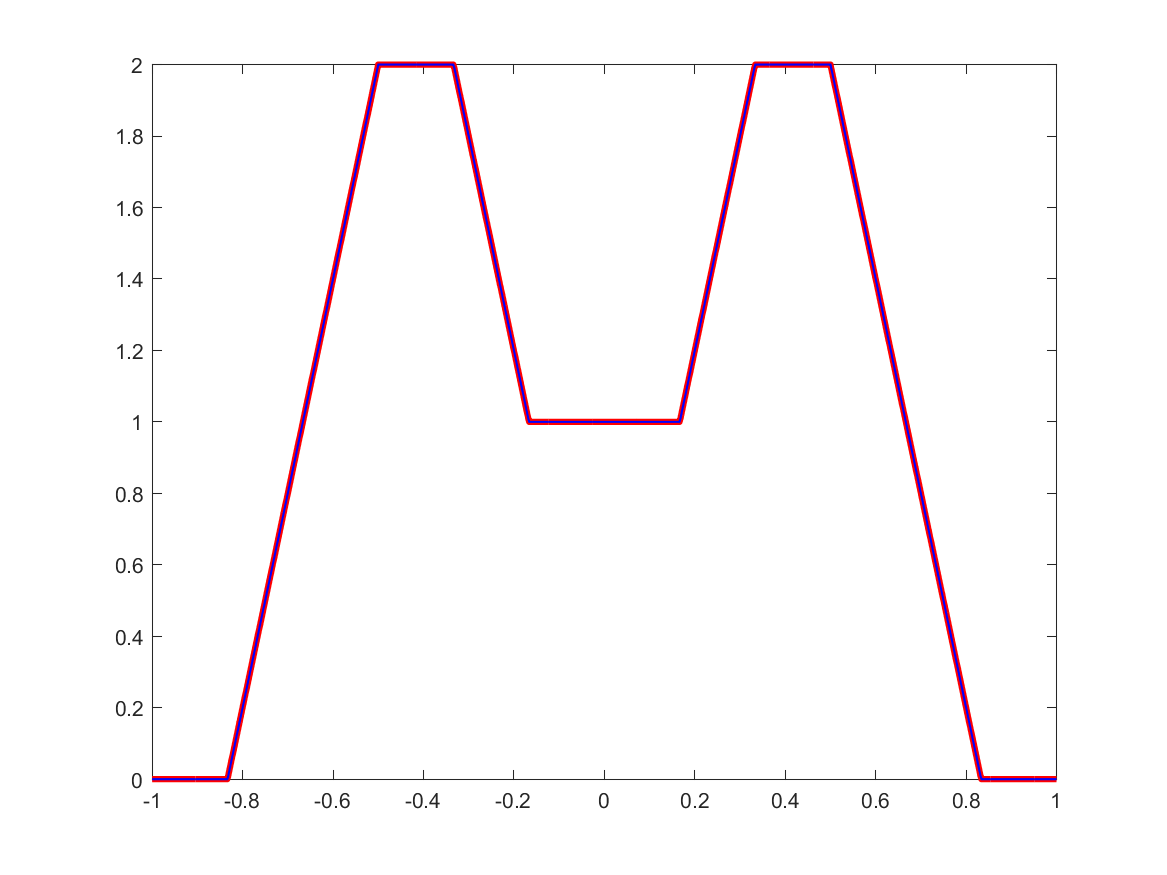
\includegraphics[trim = 50 30 50 20, clip, width=\linewidth]
      {pictures/chapExperiments/secGeneralInfo/f01Plots/exactSolutionAxis.png}
    \label{fig:f01ExactSolAxis}
  \end{subfigure} 
  \caption{Eingangssignal $f_1$ und exakte Lösung $u_1$ sowie deren
  Darstellungen entlang der x-Achse (blau) und der y-Achse (rot) für
  $\alpha=1$.}
  \label{fig:f01Plots}
\end{figure}

Ableitung von u wird zu Berechung von E(u) gebraucht nochmal sagen, sonst 
irrelevant für Experimt

vielleicht ,der Gradient von u ist\ldots, damit approximieren wir die
exakte Energie \ldots)

Nach \Cref{sec:constructionInputSignal} lauten die entsprechenden Ableitungen
\begin{align*}
  \partial_r f_1(r)
  &=
  \begin{cases}
    108,
    & \text{falls } r\in\left[0,\frac{1}{6}\right],\\
    6\alpha\beta(6r-1)^{\beta-1} +\frac{1}{r^2}, 
    & \text{falls } r\in\left(\frac{1}{6},\frac{1}{3}\right],\\
    \left(36\pi^2+\frac{1}{r^2}\right)\cos(\pi(6r-2))
    + \frac{6\pi}{r}\sin(\pi(6r-2)), 
    & \text{falls } r\in\left(\frac{1}{3},\frac{1}{2}\right],\\
    -\left(6\alpha\beta\left( \frac{5}{2}-3r \right)^{\beta-1}+
    \frac{1}{r^2}\right),
    & \text{falls } r\in\left(\frac{1}{2},\frac{5}{6}\right],\\
    -\left( \left( 18\pi^2+\frac{1}{2r^2} \right)\cos(\pi(6r-5))
    +\frac{1}{2r^2} + \frac{3\pi}{r}\sin(\pi(6r-5))\right), 
    &\text{falls } r\in\left(\frac{5}{6},\infty\right),
  \end{cases}\\
  \partial_r u_1(r) 
  &= 
  \begin{cases}
    0,
    & \text{falls } r\in\left[0,\frac{1}{6}\right],\\
    6\beta(6r-1)^{\beta-1}, 
    & \text{falls } r\in\left(\frac{1}{6},\frac{1}{3}\right],\\
    0, 
    & \text{falls } r\in\left(\frac{1}{3},\frac{1}{2}\right],\\
    -6\beta\left( \frac{5}{2}-3r \right)^{\beta-1},
    & \text{falls } r\in\left(\frac{1}{2},\frac{5}{6}\right],\\
    0,
    &\text{falls } r\in\left(\frac{5}{6},\infty\right).
  \end{cases}
\end{align*}



Ein Problem mit unstetigem Eingangssignal legen wir besonderes
Augenmerk auf das Graufarbenbild \texttt{cameraman} aus \cref{fig:cameraman}
als Eingangssignal. 

[nach cameraman Erwähnung] Auch für dieses Beispiel, das stark unregulär ist,
haben selbst deutlich höhere Integrationsgrade als 10 zu keinen veränderten
Raten geführt. 
Auch geringere nicht, da aber alle Methoden, die \texttt{integrate} aufrufen
werden vor oder nach der primalen-dualen Iteration aufgerufen, 
beeinflusst dies die Laufzeit nicht negativ und wird so gewählt um möglichst
exakte Integration zu gewährleisten.

Als initiale Geometrie nutzen wir dafür entsprechend immer
\texttt{BigSquare} des AFEM-Pakets (vlt. verweis auf Package falls vorhanden)
ohne initiale Rotverfeinerung [Abbildung mit der Triangilierung linken], da
diese den Einheitskreis enthält.
Fur dieses nutzen wir als initiale
Triangulierung für das erste Level des AFEM Algs die Triangulierung
\texttt{Square} [mach so wie eben] [s. Abb \ldots].

\begin{figure}[!ht]
  \centering
  \begin{subfigure}[b]{.48\linewidth}
    \caption{\texttt{BigSquare}}
    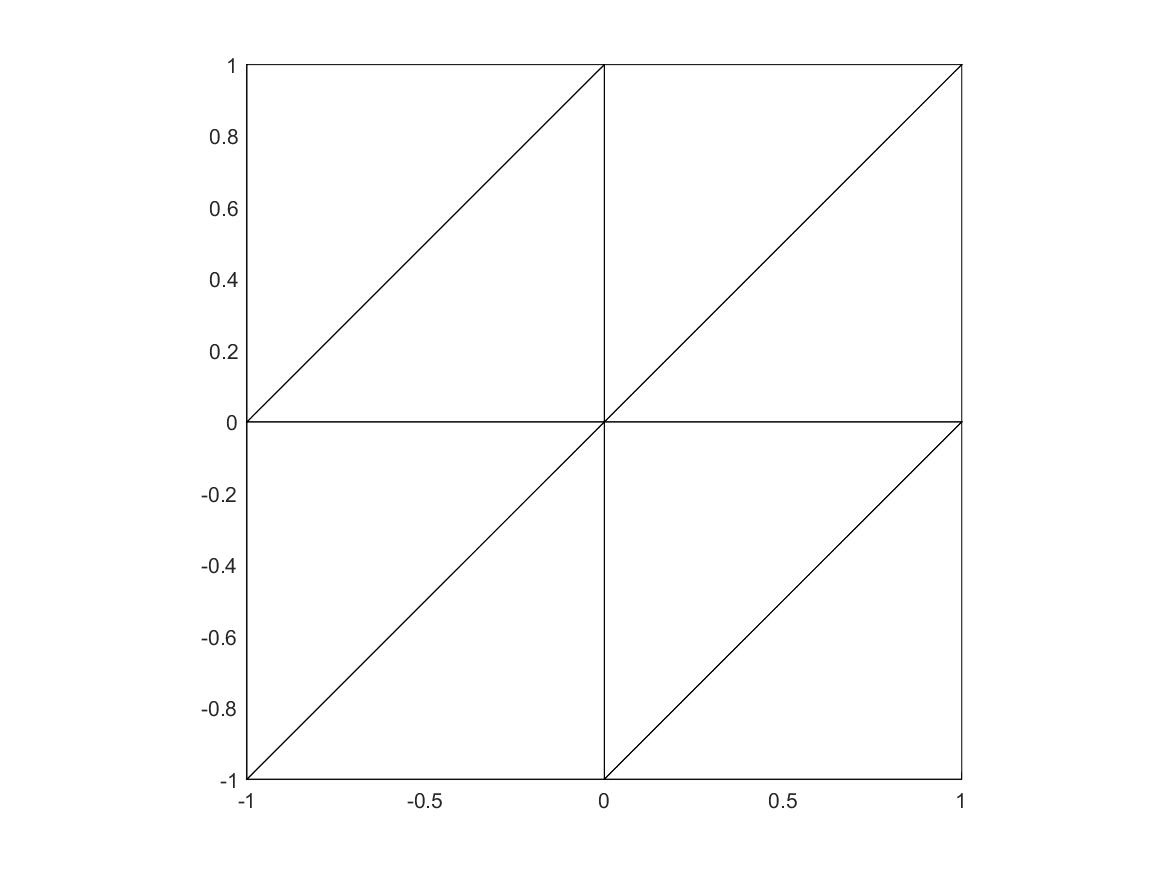
\includegraphics[trim = 90 30 90 20, clip, width=\linewidth]
      {pictures/chapExperiments/secGeneralInfo/bigSquareTriang.png}
    \label{fig:triangBigSquare}
  \end{subfigure}
  \quad
  \begin{subfigure}[b]{.48\linewidth}
    \caption{\texttt{Square}}
    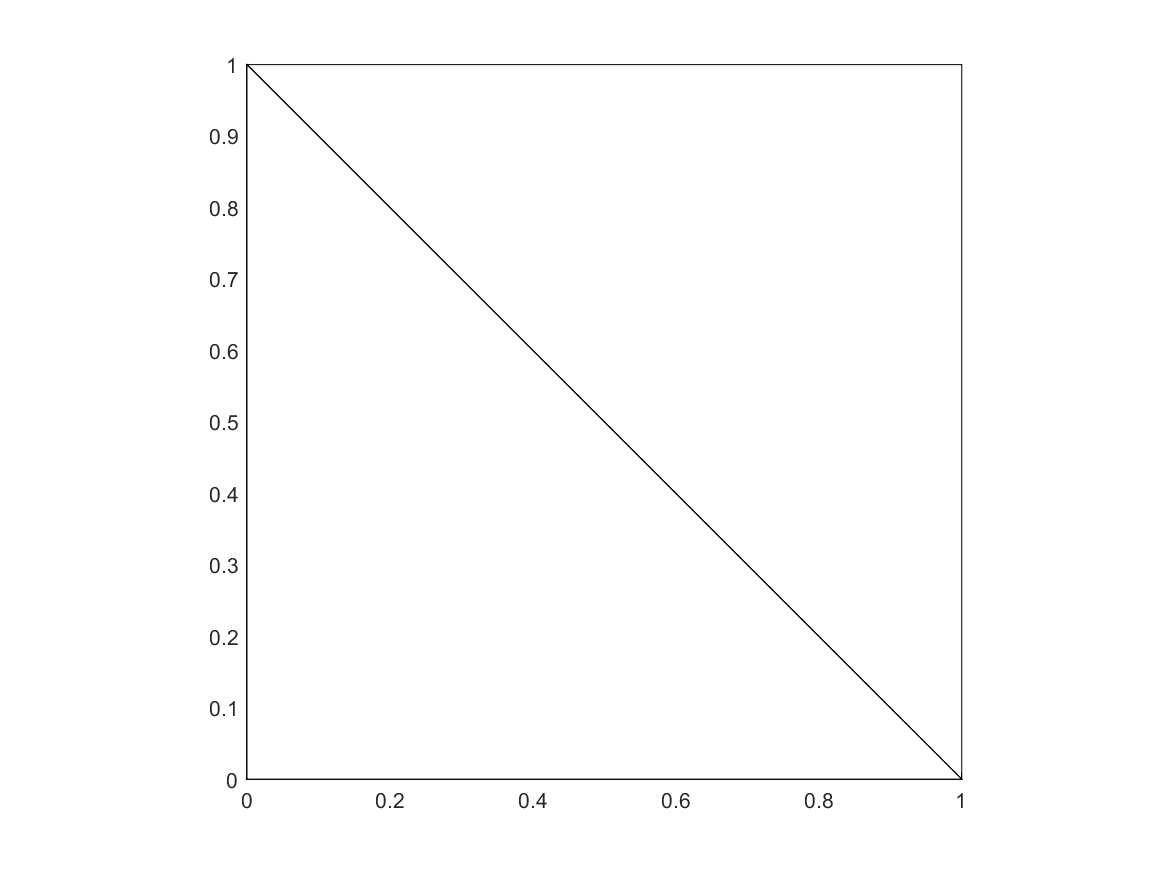
\includegraphics[trim = 90 30 90 20, clip, width=\linewidth]
      {pictures/chapExperiments/secGeneralInfo/squareTriang.png}
    \label{fig:triangSquare}
  \end{subfigure}
  \caption{In den Experimenten genutzte initiale Triangulierung.}
  \label{fig:initialTriangulations}
\end{figure}

Führen wir eines der Experimente mit adaptiver Netzverfeinerung durch, so
wählen wir den Bulk-Parameter für den Mark-Schritt des AFEM-Algorithmus, soweit
nicht anders angegeben, $\theta=0.5$.
Auf die Wahl der Parameter $\tau$ und $\epsstop$ für die primale-duale
Iteration werden wir im folgenden Abschnitt [ref] eingehen.
Zur Wahl des Parameters $\gamma$ auf dem Verfeinerungsindikator betrachten
wir in Abschnitt (Experimente mit exakter Lösung) ein.

  überlegen, welche Parmeter für jedes Experiment nochmal gesagt werden sollen
  definitiv: 

\section{Wahl der Parameter für die primale-duale Iteration}
alles zu tau mit hypothesse

beispiel ohne konvergenz aufzeigen und dafür auch die Triangulierung zeigen

zu abbruchkriterium

zu gamma (0, 0.5, 1) noch irgendwo ein Experiment mit Info, dass 0 und 1e-4 oder
so was identisch sind


\section{Experimente mit bekannter exakter Lösung}

f01 vor allem

hier vielleicht auch einmal einwerfen, wie die Iteration konvergiert
(vlt auch in der vorigen Section, im Vergleich zu den schlechten Wahlen,
die dort auch getroffen werden.

dann abschweif zu höhere Regularität

hier eventuell auch experimte für AFEM Params?

dann insgesamt raten abarbeiten und interpretieren

\section{Graufarbenbilder als Eingangssignale}
cameraman

abschweif zu denoise example aus intro hier erklären

zum abschluss zu approximation von white circle mit stetigeer funktion (plots
dementsprechend

\section{Fazit und Ausblick}

%%%%% hiervor finalized
%%%%% ab hier Skizze

Dazu gehört ein Beispiel mit bekannter Lösung, das wir nach cite(section)
konstruieren, ein komplexes Beispiel ohne Lösung mit einer unstetigen Funktion,
hier ein Bild als Eingangssignal und eine einfache, diskontinuierliche Funktion
als Eingangssignal und eine, ebenfalls nach section konstruierte stetige 
Approximation dieser.

\todo[inline]{Neue Gliederung: vgl Storn oder noch besser Sophie, statt
Auswertung ,Zusammenfassung und Ausblick'. Oder einfach wie Franz, ohne
Zsmfssg, ,Numerische Experimente und SChlussfolgerung' oder so}


Alle Allgemeinen Infos unter die Hauptüberschrift, keine eigene Section,
da auch integrate gleich 10 erwähnen



Mache alle mögliche Sachen, prüfe Dinge die gelten sollen. Für ein
Beispiel (z.B. CCs) fange mit basics an, also mal an einem Iterationsplot
aufzeigen, dass die Energie tatsächlich von oben gegen was konvergiert und 
gehe dann weiter zu anderen Themen wie den Raten, GLEB etc.

\todo[inline]{Probiere auch thm:convexity irgendwie informell zu erwähnen ,,wir
sehen, dass sogar ohne die Sprünge das stimmt\ldots`` oder so}

\todo[inline]{in chap 6 cf.s auf integrate etc nicht ständig sonder einmal 
gesammelt am Anfang oder drauf achten, dass das nur beim ersten Erwähnen zitiert 
wird}

\todo[inline]{Programm gibt Sprungtermsumme aus, z.B. stagnierend bei 11 auf
allen Leveln, darauf vielleicht noch kurz in der Auswertung eingehen ,man
sieht, dass die Sprünge tatsächlch im nonkonformen Problem nicht minimiert
werden oder so'}




Zuerst allgemeines, alle Infromationen, die ggf bei allen Experimten in den 
folgenden Abschnitten immer gleich sind und möglicherweise kurze Kommentare,
warum diese entspreched gewählt sind.

\bigskip

Alle Experimentparameter die stets gleich gesetzt sind Eingangs einmal erwähnen,
insbesondere degree4Integrate, was immer als 10 gesetzt wird, mit ähnlichem 
Kommentar wie PB auf S 30


\bigskip

Bei Beschreibung wie die Bilder der Einleitung zur Rauschunterdrückung
entstanden sind auch erwähnen, dass $f=\alpha g$ eine Rolle spiele usw.


%%%%%%%%%%%%%%%%%%%%%%%%%%%%%%%%%%%%%%%%%%%%%%%%%%%%%%
\todo[inline]{Beschreibe hier nur das allgemeine Vorgehen und die 
mathematischen Hintergründe und schreibe die genutzten Beispiele an
entsprechender Stelle in Numerische Beispiele oder so. Die ungenutzten Beispiele 
die trotzdem im Ordner liegen können in einem extra Abschnitt aufgezählt werden}
Schema ist dann: Nach section Konstruktion einer exakten Lösung erhalten wir
für die Wahl u mit sgn bla die rechte Seite f.
Die Details bei bestimmten Konstruktionen, etwa ,,um H2 zu erhalten fordern wir
noch`` ergänzen beim Vorstellen des entsprechenden Experimentes, hier nur das 
allgemeinste, das, was CC wirklich geschrieben hat.
%%%%%%%%%%%%%%%%%%%%%%%%%%%%%%%%%%%%%%%%%%%%%%%%%%%%%%
Wir wollen damit Experimente konstruieren um Aussagen in \ldots oder \ldots
zu prüfen, entsprechend müssen wir noch fordern
Da in den Kapiteln GLEB und bla u in H10 relevant wird, fordern wir
weiterhin \ldots
%%%%%%%%%%%%%%%%%%%%%%%%%%%%%%%%%%%%%%%%%%%%%%%%%%%%%%


Für die Funktion
\begin{align*}
  u_2(r)\coloneqq 
  \begin{cases}
    1, & \text{wenn } 0\leq r\leq\frac{1-\beta}{2},\\
    -\frac{1}{\beta}r + \frac{1+\beta}{2\beta}, & 
    \text{wenn } \frac{1-\beta}{2}\leq r\leq \frac{1+\beta}{2},\\
    0, & \text{wenn } \frac{1+\beta}{2}\leq r,
  \end{cases}
\end{align*}
erhält man mit der Wahl
\begin{align*}
  \sgn&(\partial_r u_2(r)) \\
  &\coloneqq 
  \begin{cases}
    \frac{4}{1-\beta}r\left(\frac{1}{1-\beta}r -1\right), &
    \text{wenn } 0\leq r\leq\frac{1-\beta}{2},\\
    -1, & \text{wenn } \frac{1-\beta}{2}\leq r\leq \frac{1+\beta}{2},\\
    \frac{4}{(\beta-1)^3}
    \left( 4r^3-3(\beta+3)r^2 +6(\beta+1)r-3\beta-1\right), & 
    \text{wenn } \frac{1+\beta}{2}\leq r\leq 1,
  \end{cases}
\end{align*}
die rechte Seite
\begin{align*}
  f_2(r)\coloneqq 
  \begin{cases}
    \alpha - \frac{4}{1-\beta}\left(\frac{3}{1-\beta}r - 2\right), &
    \text{wenn } 0\leq r\leq\frac{1-\beta}{2},\\
    -\frac{\alpha}{\beta}\left( r-\frac{1+\beta}{2} \right) +\frac{1}{r}, & 
    \text{wenn } \frac{1-\beta}{2}\leq r\leq \frac{1+\beta}{2},\\
    \frac{-4}{(\beta-1)^3}
    \left( 16r^2 -9(\beta+3)r + 12(\beta+1) - \frac{3\beta+1}{r}\right), & 
    \text{wenn } \frac{1+\beta}{2}\leq r\leq 1.
  \end{cases}
\end{align*}

Es folgen zwei Beispiele mit exakter Lösung $u_3=u_4 \in H^2_0((0,1)^2)$, 
gegeben durch 
\begin{align*}
  u_3(r)=u_4(r)\coloneqq 
  \begin{cases}
    1, & \text{wenn } 0\leq r\leq\frac{1}{3},\\
    54r^3 - 81r^2 + 36r - 4, & 
    \text{wenn } \frac{1}{3}\leq r\leq \frac{2}{3},\\
    0, & \text{wenn } \frac{2}{3}\leq r.
  \end{cases}
\end{align*}
Mit der Wahl
\begin{align*}
  \sgn&(\partial_r u_3(r)) \\
  &\coloneqq 
  \begin{cases}
    54r^3-27r^2, & \text{wenn } 0\leq r\leq\frac{1}{3},\\
    -1, & \text{wenn } \frac{1}{3}\leq r\leq \frac{2}{3},\\
    -54r^3 + 135r^2 - 108r + 27, & \text{wenn } \frac{2}{3}\leq r\leq 1,
  \end{cases}
\end{align*}
erhalten wir die rechte Seite
\begin{align*}
  f_3(r)\coloneqq 
  \begin{cases}
    \alpha - 216r^2 + 81r, &
    \text{wenn } 0\leq r\leq\frac{1}{3},\\
    \alpha\left(54r^3 - 81r^2 + 36r - 4\right)) + \frac{1}{r}, & 
    \text{wenn } \frac{1}{3}\leq r\leq \frac{2}{3},\\
    216r^2 - 405r + 216 - \frac{27}{r}, & 
    \text{wenn } \frac{2}{3}\leq r\leq 1,
  \end{cases}
\end{align*}
für die gilt $f_3\in H^1_0$
und mit der Wahl
\begin{align*}
  \sgn&(\partial_r u_4(r)) \\
  &\coloneqq 
  \begin{cases}
    -1458r^5 + 1215r^4 - 270r^3, & \text{wenn } 0\leq r\leq\frac{1}{3},\\
    -1, & \text{wenn } \frac{1}{3}\leq r\leq \frac{2}{3},\\
    -243r^4 + 756r^3 - 864r^2 + 432r - 81, 
    & \text{wenn } \frac{2}{3}\leq r\leq 1,
  \end{cases}
\end{align*}
erhalten wir die rechte Seite
\begin{align*}
  f_4(r)\coloneqq 
  \begin{cases}
    \alpha + 8748r^4 - 6075r^3 + 1080r^2, &
    \text{wenn } 0\leq r\leq\frac{1}{3},\\
    \alpha\left(54r^3 - 81r^2 + 36r - 4\right) + \frac{1}{r}, & 
    \text{wenn } \frac{1}{3}\leq r\leq \frac{2}{3},\\
    1215r^3 - 3024r^2 + 2592r - 864 + \frac{81}{r}, & 
    \text{wenn } \frac{2}{3}\leq r\leq 1,
  \end{cases}
\end{align*}
für die gilt $f_4\in H^2_0$.


\begin{align*}
  \partial_r f_2(r) &= 
  \begin{cases}
    -\frac{12}{(1-\beta)^2},&\text{wenn }0\leq r\leq\frac{1-\beta}{2},\\
    -\frac{\alpha}{\beta}-\frac{1}{r^2},&
    \text{wenn } \frac{1-\beta}{2}\leq r\leq \frac{1+\beta}{2},\\
    -\frac{4}{(1-\beta)^3}\left( 32r-9(\beta+3)+\frac{3\beta+1}{r^2} \right),&
    \text{wenn } \frac{1+\beta}{2}\leq r\leq 1,\\
  \end{cases}\\
  \partial_r u_2(r) &= 
  \begin{cases}
    0,&\text{wenn }0\leq r\leq\frac{1-\beta}{2},\\
    -\frac{1}{\beta},&
    \text{wenn } \frac{1-\beta}{2}\leq r\leq \frac{1+\beta}{2},\\
    0,&\text{wenn } \frac{1+\beta}{2}\leq r,
  \end{cases}\\
  \partial_r f_3(r) &=
  \begin{cases}
    - 432r + 81, & \text{wenn } 0\leq r\leq\frac{1}{3},\\
    \alpha\left(162r^2 - 162r + 36\right) - \frac{1}{r^2}, & 
    \text{wenn } \frac{1}{3}\leq r\leq \frac{2}{3},\\
    432r - 405 + \frac{27}{r^2}, & 
    \text{wenn } \frac{2}{3}\leq r\leq 1,
  \end{cases}\\
  \partial_r f_4(r) &=
  \begin{cases}
    34992r^3 - 18225r^2 + 2160r, & \text{wenn } 0\leq r\leq\frac{1}{3},\\
    \alpha\left(162r^2 - 162r + 36\right) - \frac{1}{r^2}, & 
    \text{wenn } \frac{1}{3}\leq r\leq \frac{2}{3},\\
    3645r^2 - 6048r + 2592 - 864 - \frac{81}{r^2}, & 
    \text{wenn } \frac{2}{3}\leq r\leq 1,
  \end{cases}\\
  \partial_r u_{3,4}(r) &=
  \begin{cases}
    0, & \text{wenn } 0\leq r\leq\frac{1}{3},\\
    162r^2 - 162r + 36, & 
    \text{wenn } \frac{1}{3}\leq r\leq \frac{2}{3},\\
    0, & \text{wenn } \frac{2}{3}\leq r\leq 1,
  \end{cases}\\
\end{align*}
